\chapter{Modelo de Requisitos}
\label{modelo_requisitos}

El modelo de requisitos es un pilar importante para garantizar que la funcionalidad implementada es de interés para un actor específico. se emplea el mecanismo de casos de uso para describir la funcionalidad para describir la funcionalidad con un alto grado de abstracción técnicas. 

\section{Modelo de Casos de Uso}
\subsection{Características Generales de los Actores}

El sistema ofrece funcionalidad que es de interés para alguno de los siguientes actores (figura \ref{actores}):

\begin{itemize}
\item \textbf{Administrador}: Se encarga de la gestión de usuarios, el registro de nuevas categorías de nodos y tareas de administración tales como copias de seguridad, corrección de errores, edición de páginas, etc.
\item \textbf{Entidad de Salud}: Para la gestión especifica de un nodo tipo Entidad de Salud. Un usuario de este tipo esta confinado a la institución que crea. Para poder gestionar información de otra entidad deberá solicitar autorización a la instancia de actor dueña del registro.
\item \textbf{Servicios Médicos:} Gestiona la información de nodos tipo Servicio Médico.
\item \textbf{Especialista:} Con permisos para gestionar nodos tipo Especialista (profesionales de la salud).
\item \textbf{Profesional TIC:} Actor abstracto que agrupa los actores que gestionan información de los nodos tipo: Equipo Médico, Operador de Telecomunicaciones y Tecnología de Interconexión.
\item \textbf{Usuario General:} Usuario general de consulta. Puede generar informes pero no se le permite modificar ningún registro.
\item \textbf{Consultor:} Especificación del usuario general en donde además de consultar información tiene acceso a los módulo de tablas de análisis, agenda y blog.
\end{itemize}

\begin{figure}
 \centering
 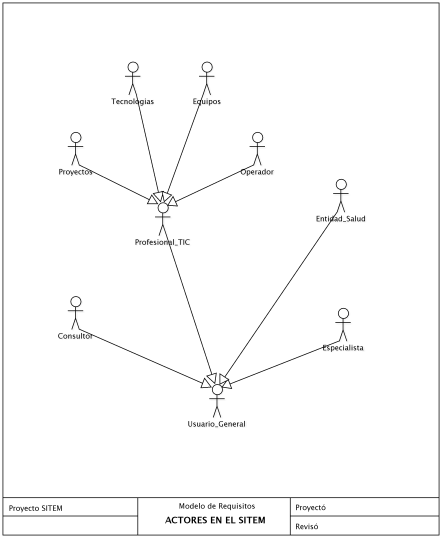
\includegraphics[width=156mm, height=182mm]{actores.png}
 \caption{Conjunto de Actores de OpenSITE;}
 \label{actores}
\end{figure}

\subsection{Casos de Usos}
Los artefactos correspondientes a los casos de uso se han empaquetado de acuerdo al tipo de nodo en el cual se desarrollan. Se incluyen solo los casos que se consideran nucleares y las especificaciones de mayor relevancia e impacto.

\begin{figure}
 \centering
 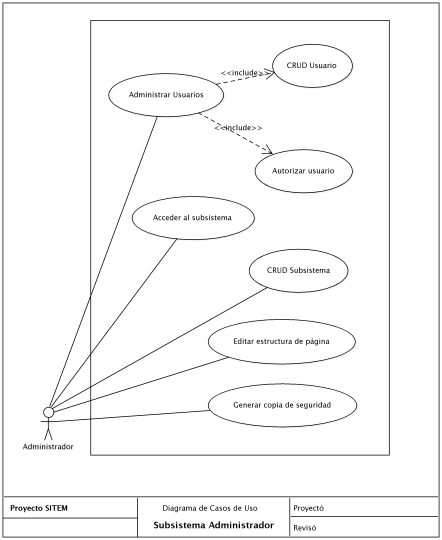
\includegraphics[width=156mm, height=182mm]{casos_admin.png}
 \caption{Casos de uso principales del Actor administrador}
 \label{casos_admin}
\end{figure}

\begin{figure}
 \centering
 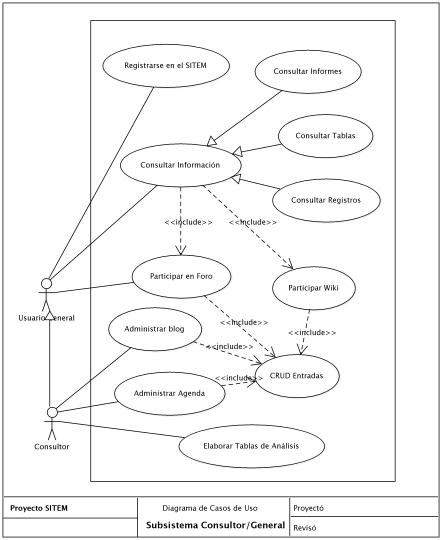
\includegraphics[width=156mm, height=182mm]{casos_consultor.png}
 \caption{Casos de uso principales del Actor Consultor/Usuario General}
 \label{casos_consultor}
\end{figure}

\begin{figure}
 \centering
 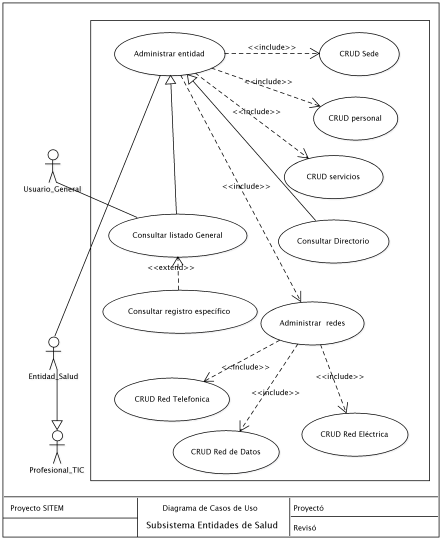
\includegraphics[width=156mm, height=182mm]{casos_entidad.png}
 \caption{Casos de uso principales del Actor Entidad de Salud}
 \label{casos_entidad}
\end{figure}

\begin{figure}
 \centering
 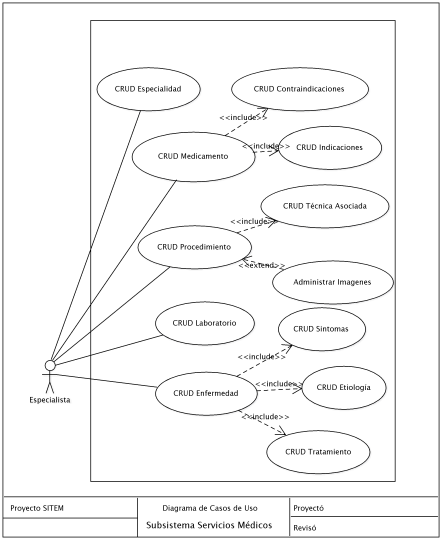
\includegraphics[width=156mm, height=182mm]{casos_servicios.png}
 \caption{Casos de uso principales del Actor Servicios Médicos}
 \label{casos_servicios}
\end{figure}

\begin{figure}
 \centering
 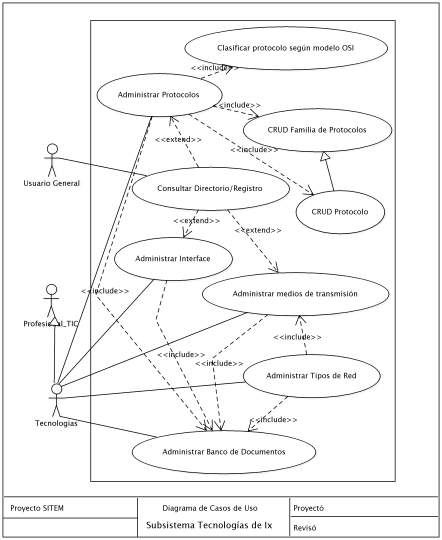
\includegraphics[width=156mm, height=182mm]{casos_tecnologias.png}
 \caption{Casos de uso principales del Actor Tecnologías de Interconexión}
 \label{casos_tecnologia}
\end{figure}

\begin{figure}
 \centering
 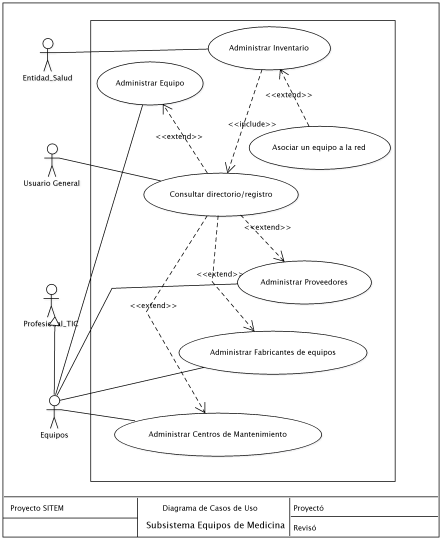
\includegraphics[width=156mm, height=182mm]{casos_equipos.png}
 \caption{Casos de uso principales en el Subsistema Equipos de Medicina}
 \label{casos_equipos}
\end{figure}

\begin{figure}
 \centering
 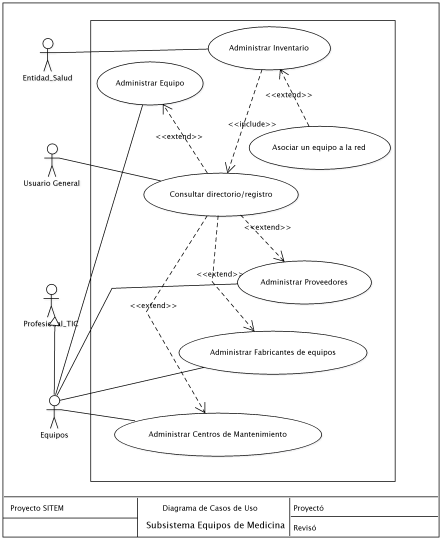
\includegraphics[width=156mm, height=182mm]{casos_equipos.png}
 \caption{Casos de uso principales en el Subsistema de Operadores de Servicios de Telecomunicaciones}
 \label{casos_telecomunicaciones}
\end{figure}
